\documentclass[11pt,a4paper]{article}
\usepackage{fullpage}
\usepackage[T1]{fontenc} 
\usepackage[utf8]{inputenc}
\usepackage{amsmath}
\usepackage{amssymb}
\usepackage{float}
\usepackage{tabularx}
\usepackage{multirow}
\usepackage{graphicx}
\usepackage{geometry}
\usepackage[table,dvipsnames]{xcolor}
\usepackage[hidelinks]{hyperref}
\usepackage[polish]{babel}
\usepackage{menukeys}
\usepackage{subcaption}

\setlength{\parindent}{0cm}
\setlength{\parskip}{2mm}
\newcolumntype{Y}{>{\centering\arraybackslash}X}
\DeclareMathOperator{\sgn}{sgn}

\begin{document}

\title{Rozpoznawanie człowieka metodami biometrii \\
\Large{
    Projekt 3. --- Rozpoznawanie na~podstawie twarzy \\
    Raport
}}
\author{Bartłomiej Dach}
\maketitle
Poniższy dokument stanowi sprawozdanie z~implementacji aplikacji dokonującej rozpoznwania człowieka na~podstawie zdjęć twarzy w~pozycji frontalnej.
W~dokumencie opisano porównywane metody oraz~zawarto wyniki eksperymentalne dla~obu metod na~dostarczonym zbiorze zdjęć.

\section{Wstęp}

Twarz to~cecha biometryczna zaliczająca~się do~cech biologicznych.
Większość mierzalnych cech twarzy (geometria, kolor skóry) jest opartych na~cechach anatomicznych lub~etnicznych.
Z~drugiej strony aspekty takie, jak~zarost czy~wiek utrudniają wykorzystanie tych~cech, ponieważ zmieniają~się z~czasem.

Rozpoznawanie na~podstawie twarzy jest częścią coraz większej liczby urządzeń konsumenckich, szczególnie w~branży urządzeń mobilnych.
Ponieważ akwizycja obrazu twarzy nie~wymaga bezpośredniego kontaktu, a~coraz~więcej smartfonów posiada kamery po~przedniej stronie, jest to wygodna metoda potwierdzenia tożsamości użytkownika telefonu.

W~ramach projektu zaimplementowano dwie metody oparte na~identyfikacji punktów charakterystycznych twarzy.
W~obu przypadkach do~znajdowania twarzy na~zdjęciach i~lokalizacji punktów charakterystycznych wykorzystano bibliotekę \texttt{dlib}.
Metody różnią~się właściwym przetwarzaniem punktów --- w jednej metodzie punkty charakterystyczne wykorzystywane~są bezpośrednio po~pewnych korekcyjnych przekształceniach geometrycznych, zaś w~drugiej w~celu porównania z~rozwiązaniami \emph{state-of-the-art} wykorzystano wytrenowany klasyfikator ResNet \cite{he2015, king2015}.
Dokładniejsze informacje znajdują~się w~podrozdziale~\ref{subsec:classification}.

\section{Opis aplikacji}

\subsection{Zastosowane biblioteki}

\begin{table}[H]
    \begin{tabularx}{\textwidth}{|r|l|X|l|c|}
        \hline
        Nr & Nazwa & Opis & Licencja & \\
        \hline
        \hline
        1 & \texttt{dlib} 19.17.0 & Biblioteka wspomagająca proces rozpoznawania twarzy & Boost & \cite{king2003} \\
        \hline
        2 & \texttt{matplotlib} 3.0.3 & Tworzenie wykresów i~wizualizacji & PSF & \cite{hunter2007} \\
        \hline
        3 & \texttt{pandas} 0.24.2 & Struktury do~manipulacji i~analizy danych & BSD & \cite{mckinney2010} \\
        \hline
        4 & \texttt{seaborn} 0.9.0 & Rozszerzone wizualizacje danych & BSD & \cite{waskom2018} \\
        \hline
        5 & \texttt{tqdm} 4.31.1 & Biblioteka wspomagająca do pasków postępu w~skryptach & MPL & \cite{dacosta2016} \\
        \hline
    \end{tabularx}
    \caption{Lista bibliotek użytych w~projekcie}
    \label{tbl:libraries}
\end{table}

\subsection{Instrukcja obsługi}
\label{sec:manual}

W~celu uruchomienia skryptów do~rozpoznawania konieczne jest zainstalowanie interpretera~Python oraz~bibliotek zawartych w~tabeli~\ref{tbl:libraries}.
Aby~zainstalować wymagane biblioteki, należy wywołać polecenie
\begin{verbatim}
$ pip3 install -r requirements.txt
\end{verbatim}
gdzie plik \texttt{requirements.txt} to~plik dołączony do~źródeł aplikacji.

\section{Opis metody}

\subsection{Rozpoznawanie twarzy na~zdjęciu}

\subsection{Lokalizacja punktów charakterystycznych}

\begin{figure}[H]
    \centering
    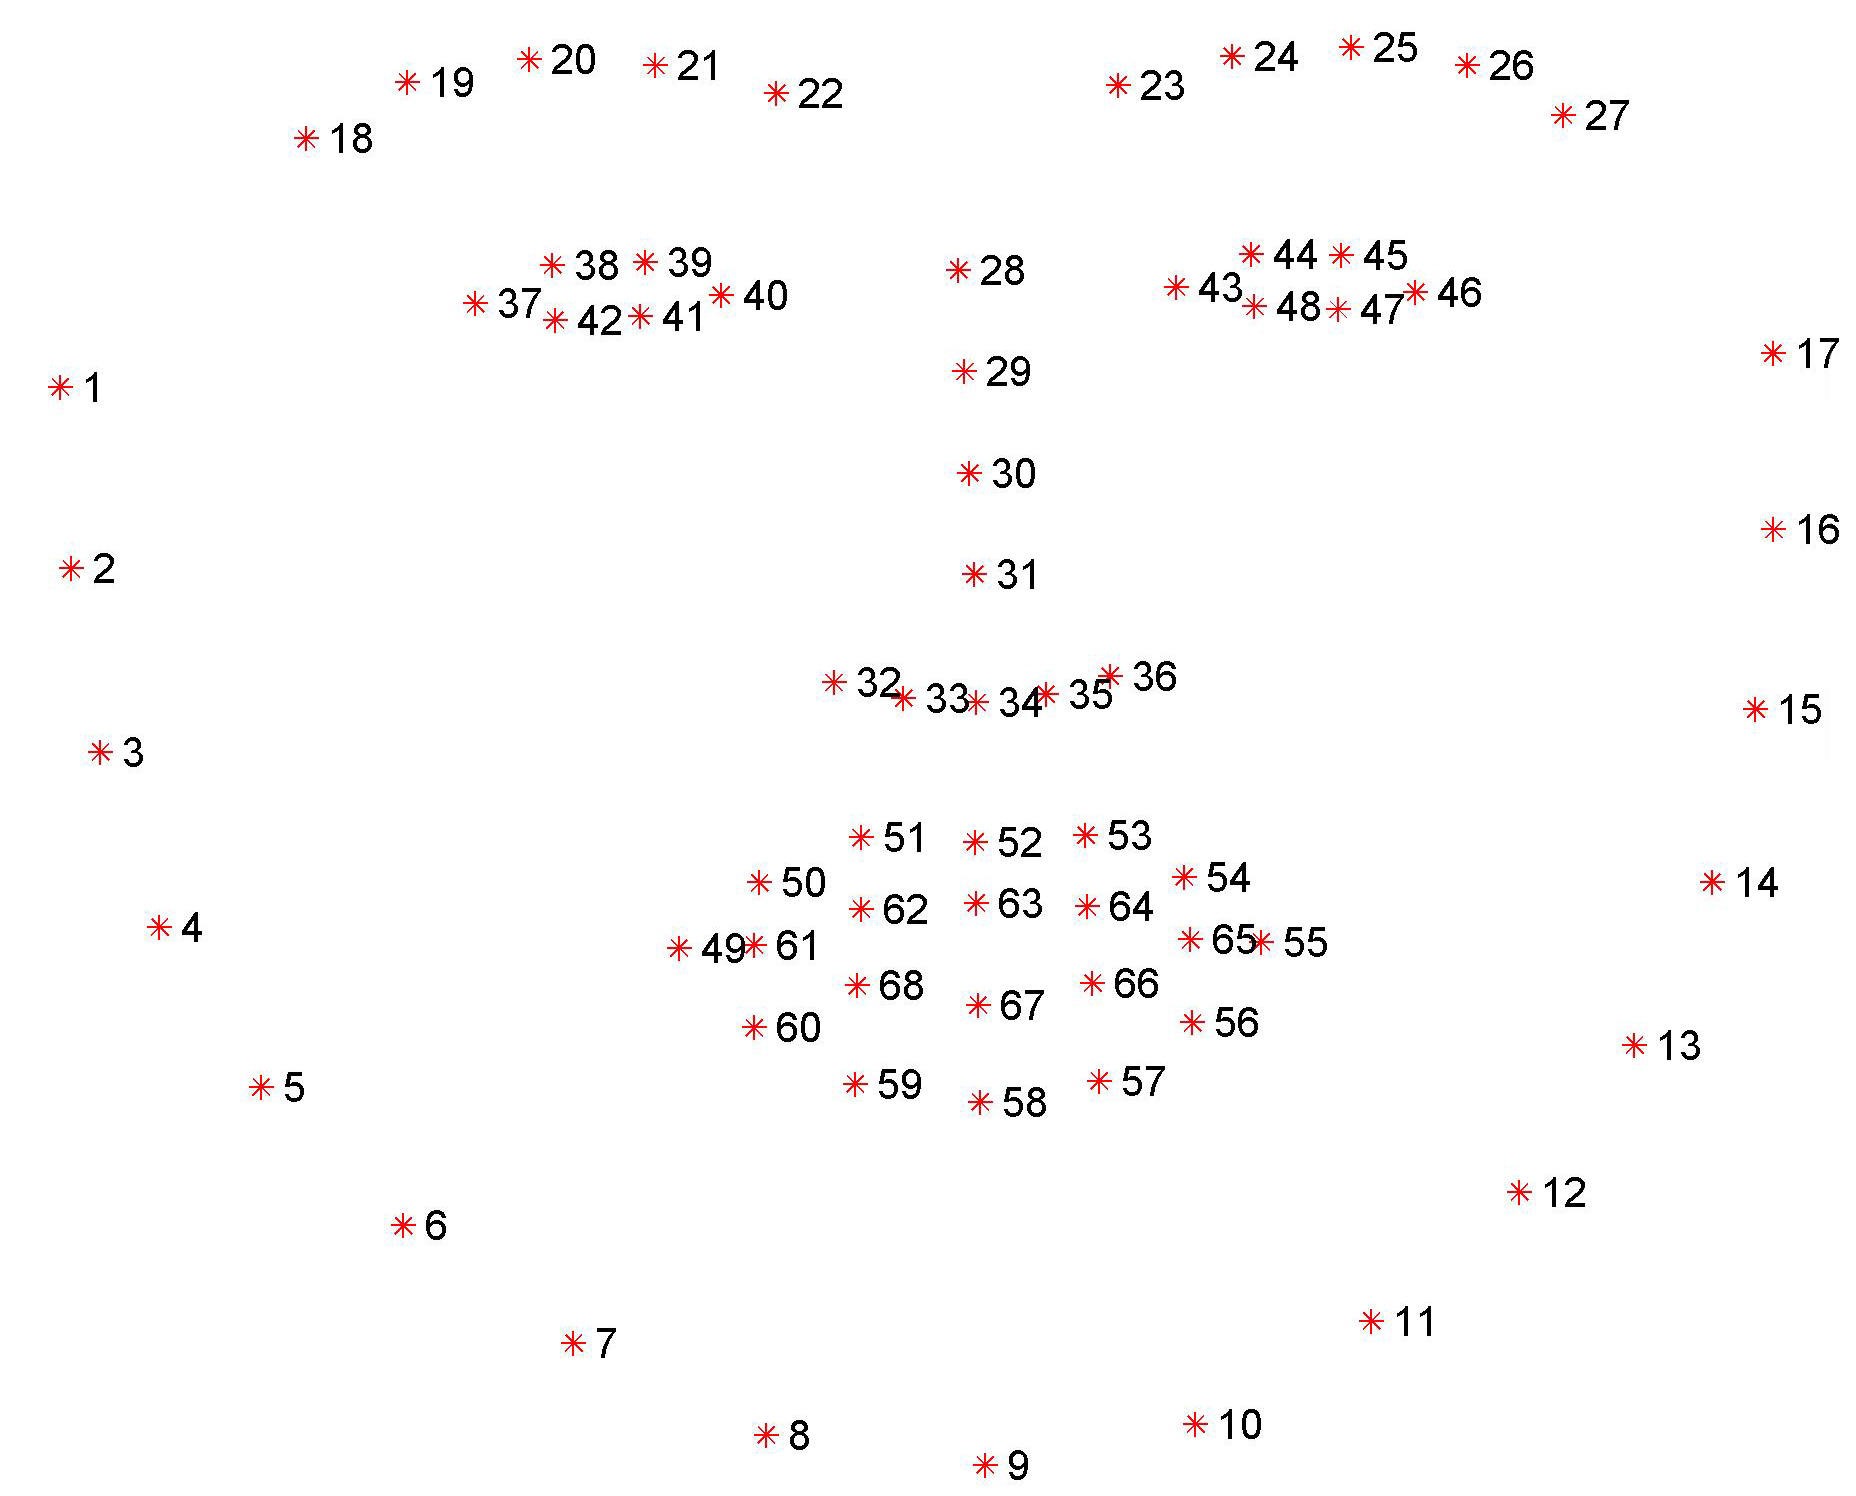
\includegraphics[width=0.6\textwidth]{res/img/figure_68_markup.jpg}
    \label{fig:68-landmarks}
    \caption{Wizualizacja 68~punktów charakterystycznych wykorzystywanych do~rozpoznawania twarzy, wytypowanych przez~\emph{Intelligent Behaviour Understanding Group}. Źródło: \cite{sagonas2013}}
\end{figure}

\subsection{Klasyfikacja twarzy na~podstawie punktów charakterystycznych}
\label{subsec:classification}

\subsubsection{Podejście normalizacyjne}

\subsubsection{Wykorzystanie klasyfikatora ResNet}

\section{Wyniki eksperymentalne}
\label{sec:results}

\begin{figure}[H]
    \begin{subfigure}{\textwidth}
        \centering
        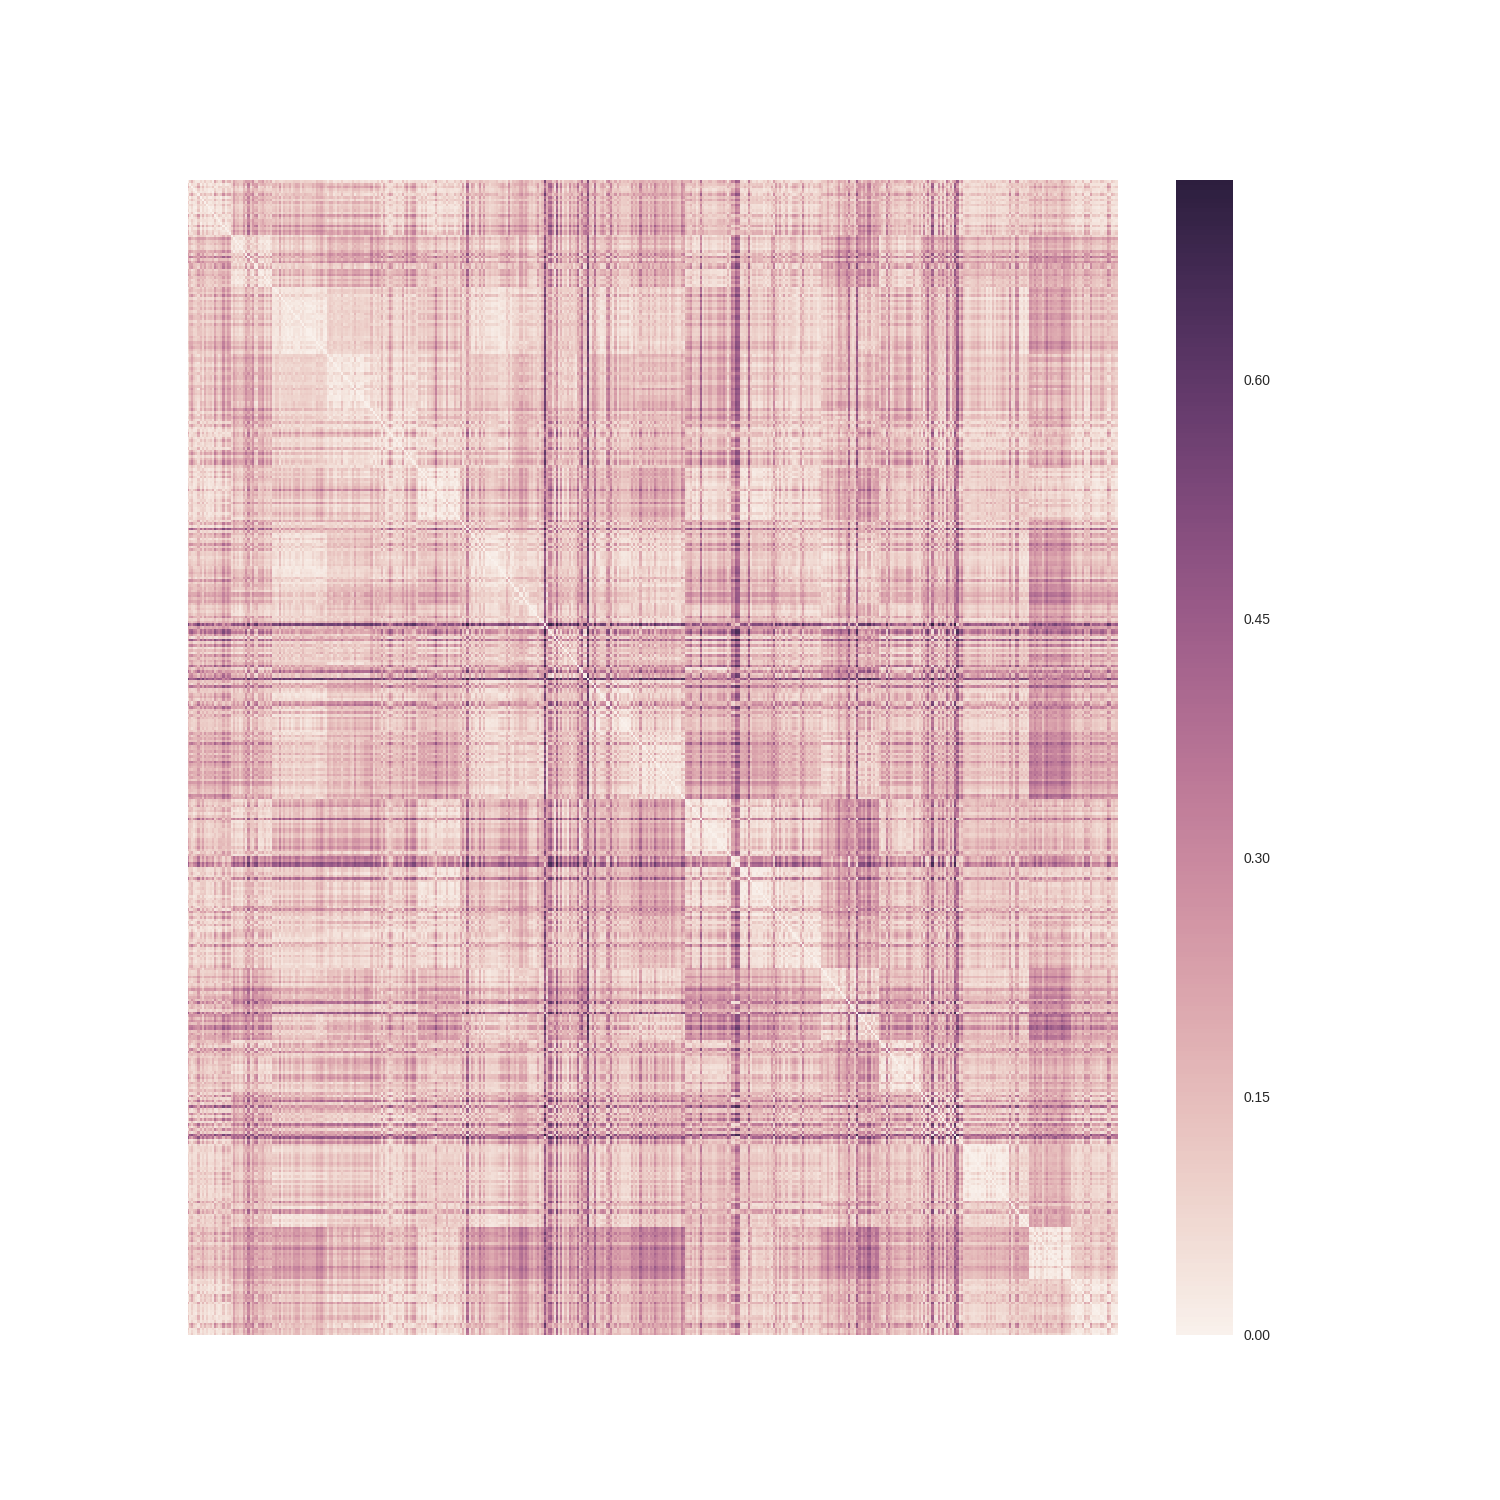
\includegraphics[width=0.6\textwidth]{res/img/normalized_distance_matrix.png}
        \label{subfig:normalized-distance-matrix}
        \caption{Macierz dla~podejścia normalizacyjnego po~przetworzeniu odległości wg~wzoru~$d' = 1 - \frac{1}{d + 1}$.}
    \end{subfigure}
    \\
    \begin{subfigure}{\textwidth}
        \centering
        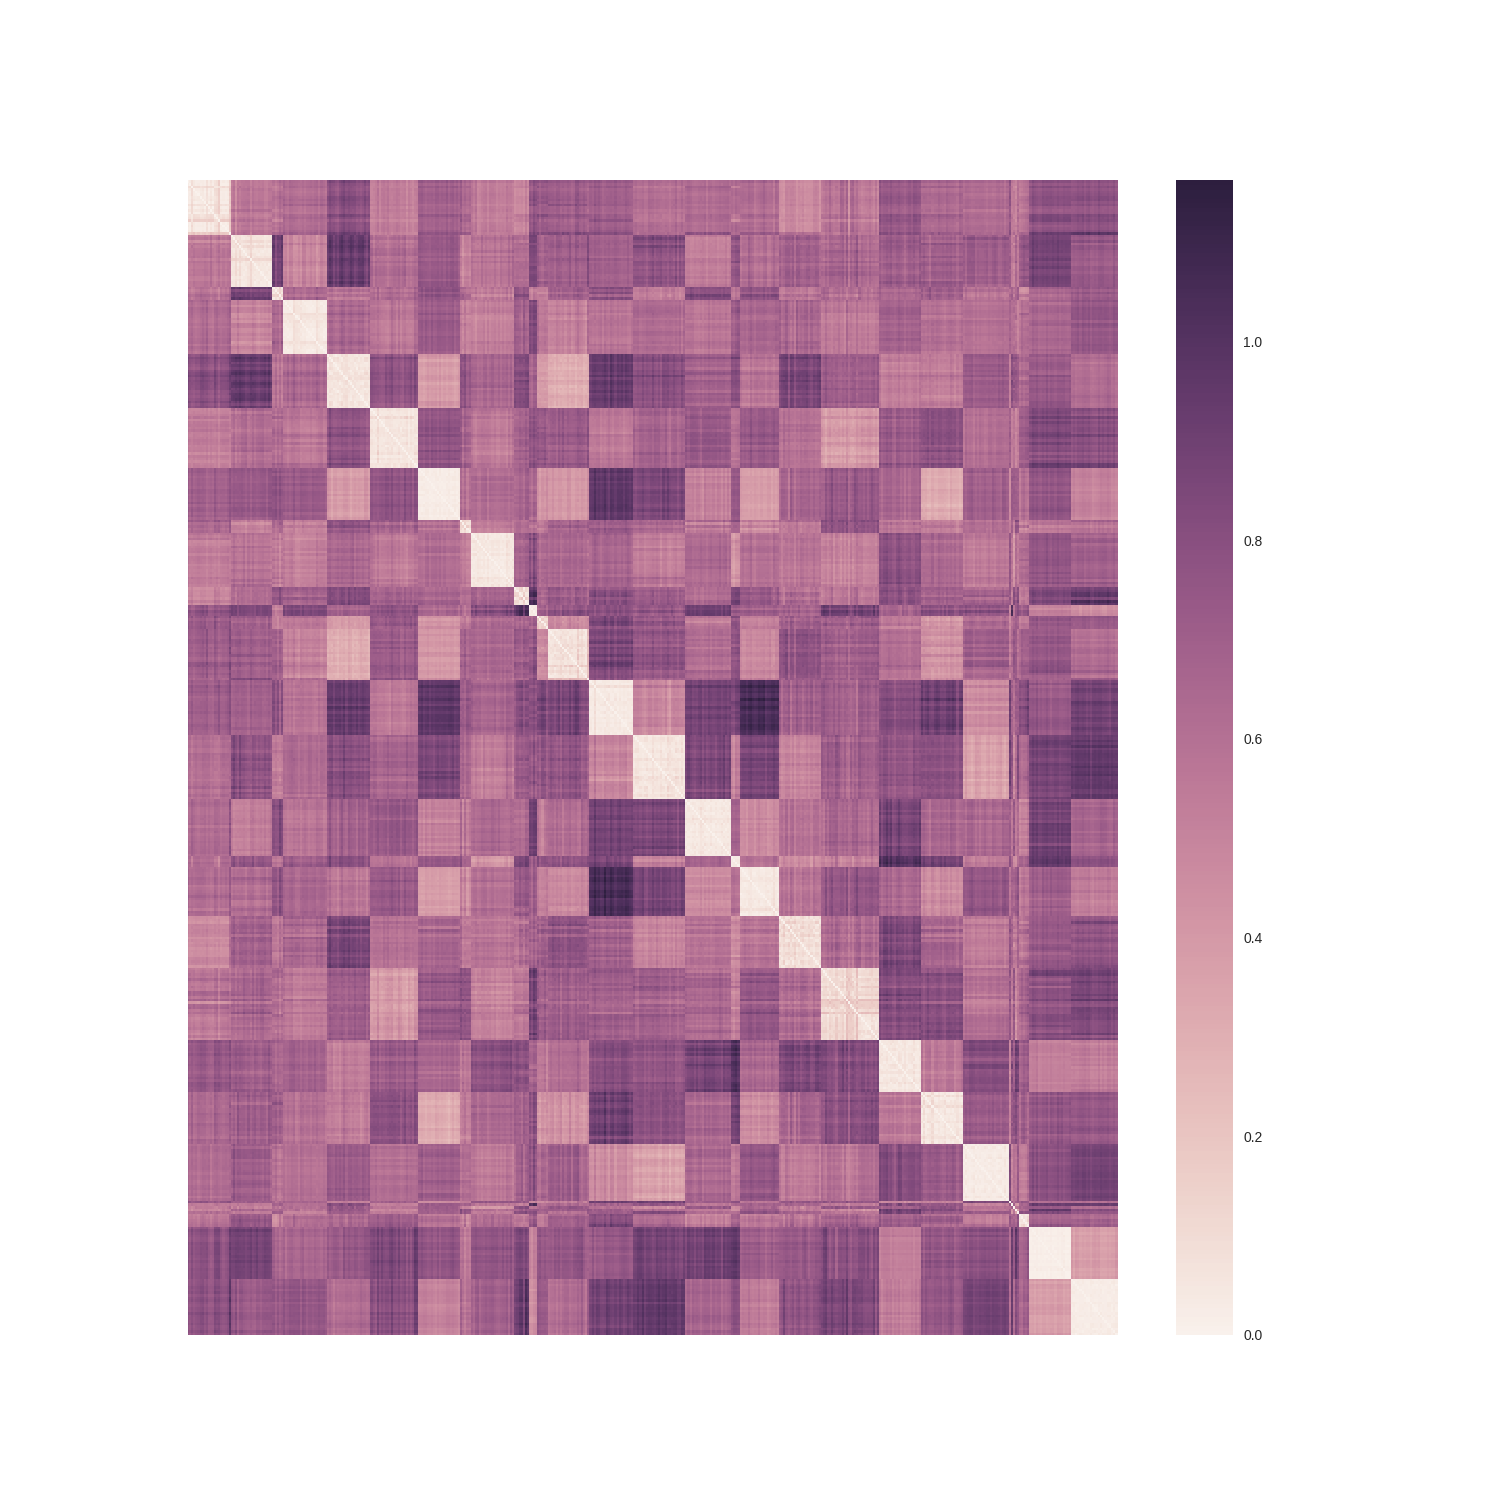
\includegraphics[width=0.6\textwidth]{res/img/resnet_distance_matrix.png}
        \label{subfig:resnet-distance-matrix}
        \caption{Macierz dla~klasyfikatora ResNet.}
    \end{subfigure}
    \caption{Macierze wzajemnych odległości dla~poszczególnych par obrazów ze~zbioru testowego.
    Zauważalne są ciemniejsze bloki wzdłuż~przekątnej, obrazujące podobieństwo wielu obrazów przedstawiających jedną osobę.}
\end{figure}

\begin{figure}[H]
    \begin{subfigure}{\textwidth}
        \centering
        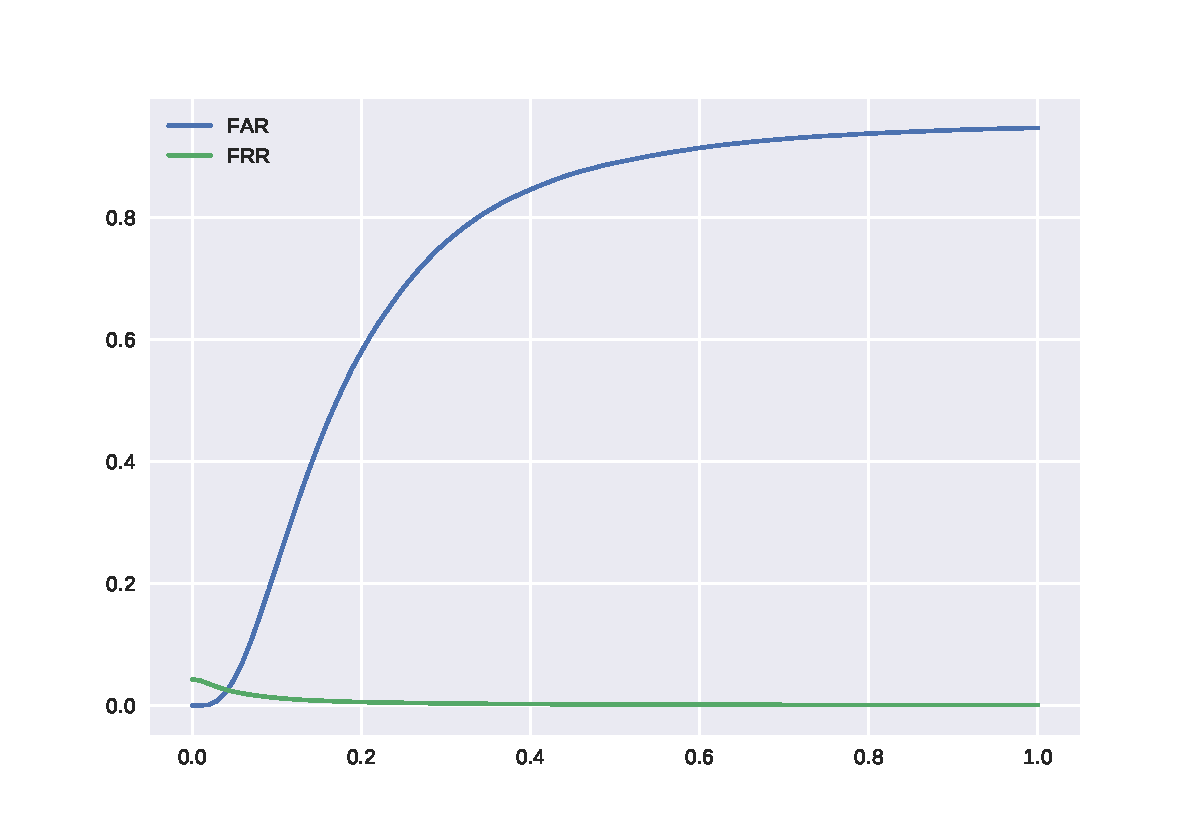
\includegraphics[width=0.8\textwidth]{res/img/normalized_error_rates.pdf}
        \label{subfig:normalized-error-rates}
        \caption{Wskaźniki FAR i~FRR dla~podejścia normalizacyjnego.}
    \end{subfigure}
    \\
    \begin{subfigure}{\textwidth}
        \centering
        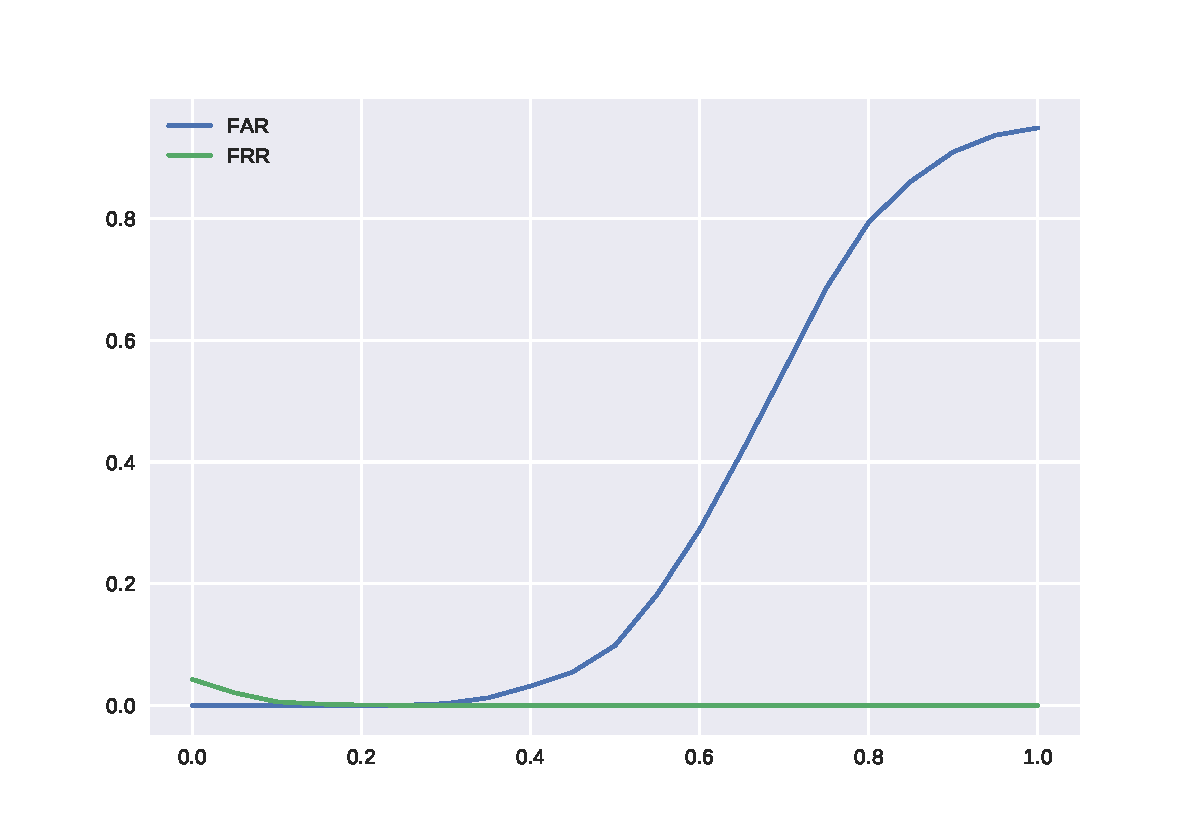
\includegraphics[width=0.8\textwidth]{res/img/resnet_error_rates.pdf}
        \label{subfig:resnet-error-rates}
        \caption{Wskaźniki FAR i~FRR dla~klasyfikatora ResNet.}
    \end{subfigure}
    \caption{Wartości wskaźników FAR i~FRR w~zależności od~przyjętego progu klasyfikacji w~zadaniu weryfikacji tożsamości na~podstawie par zdjęć.}
\end{figure}

\begin{figure}[H]
    \begin{subfigure}{\textwidth}
        \centering
        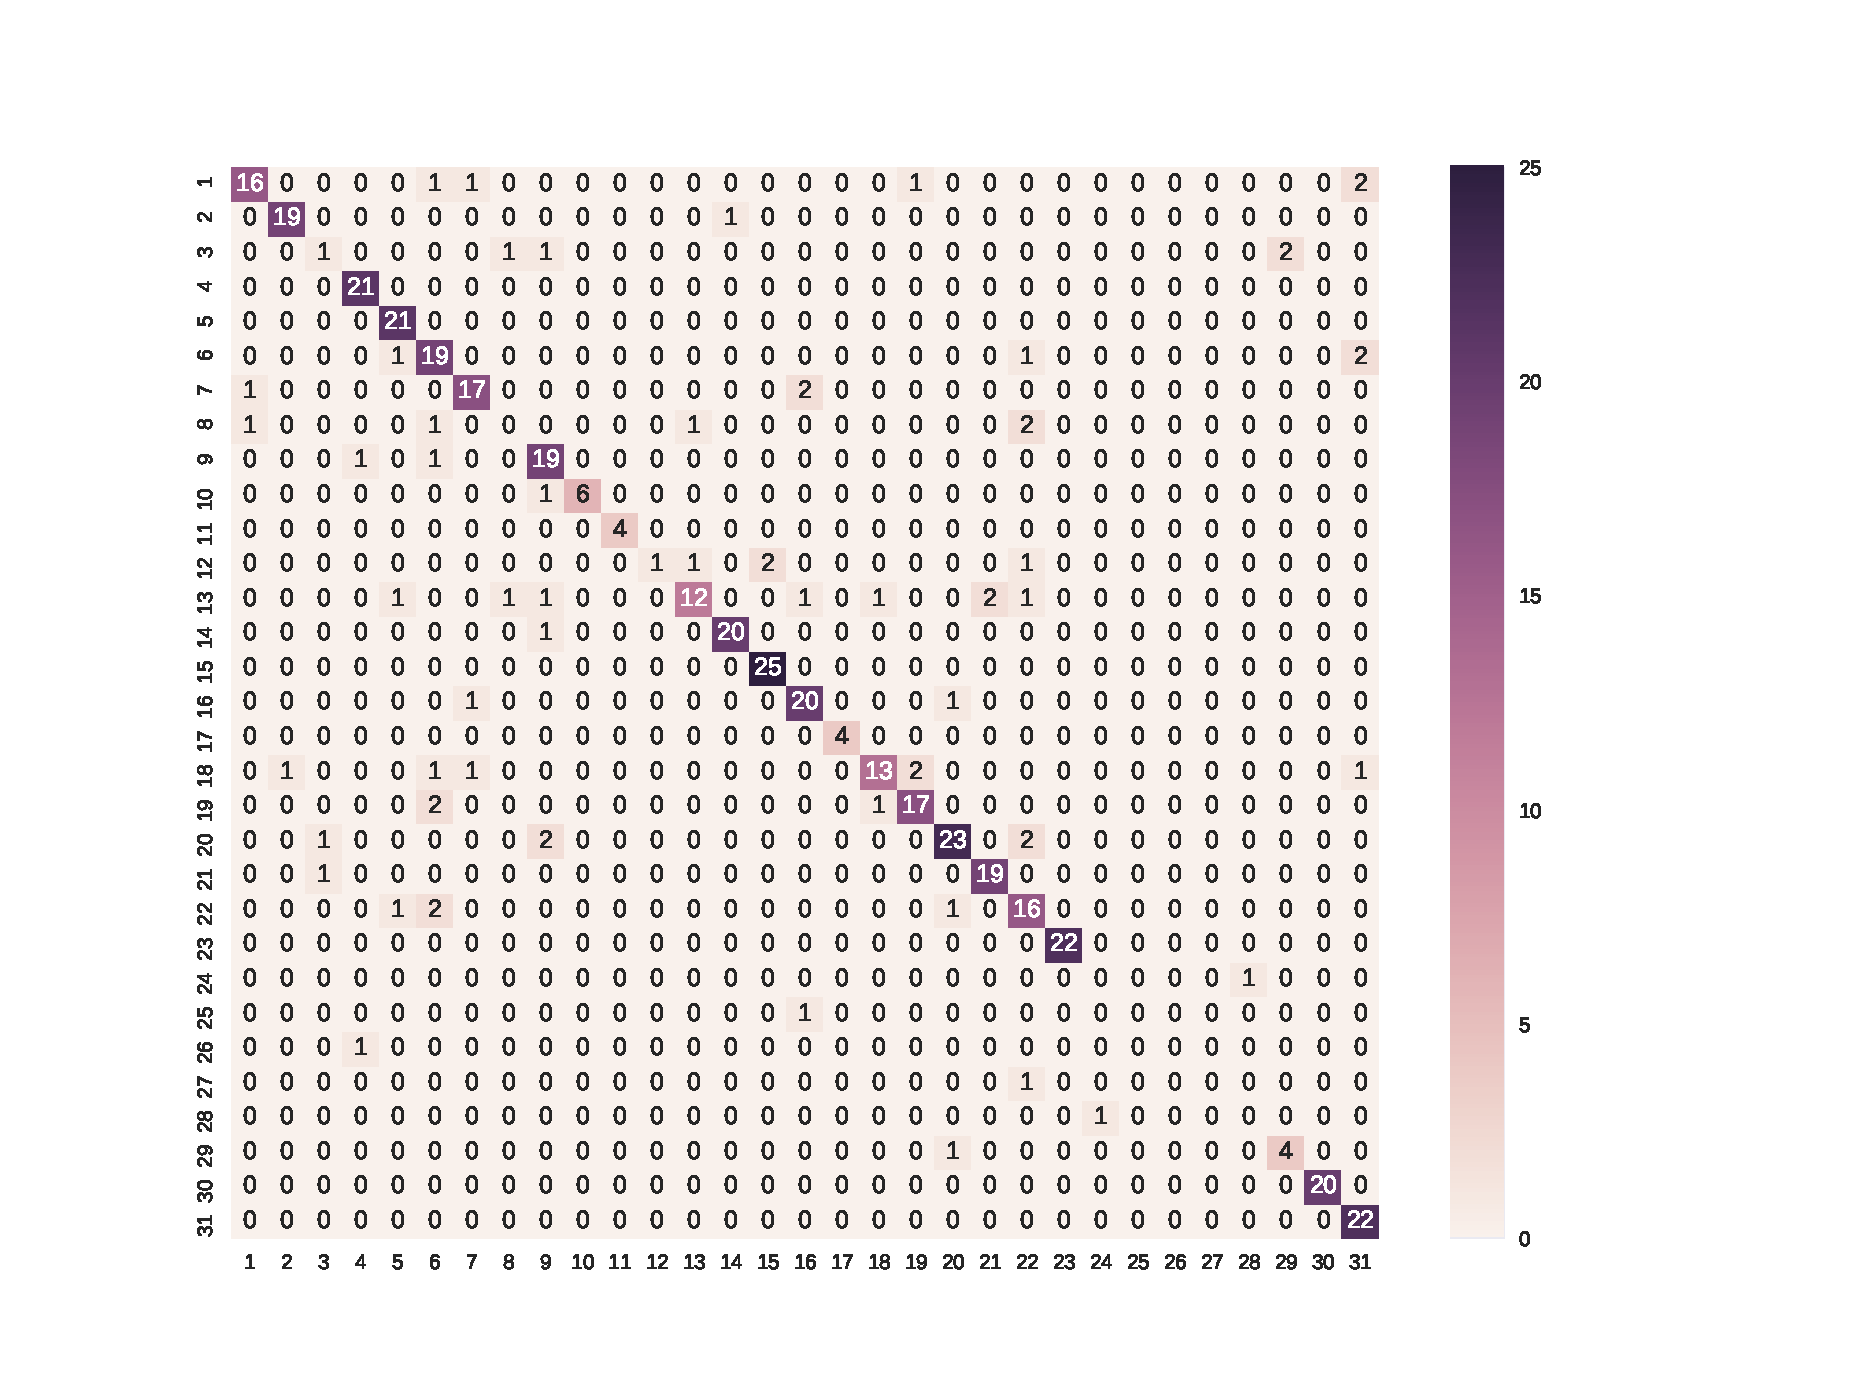
\includegraphics[width=0.8\textwidth]{res/img/normalized_confusion_matrix.pdf}
        \label{subfig:normalized-distance-matrix}
        \caption{Macierz dla~podejścia normalizacyjnego.}
    \end{subfigure}
    \\
    \begin{subfigure}{\textwidth}
        \centering
        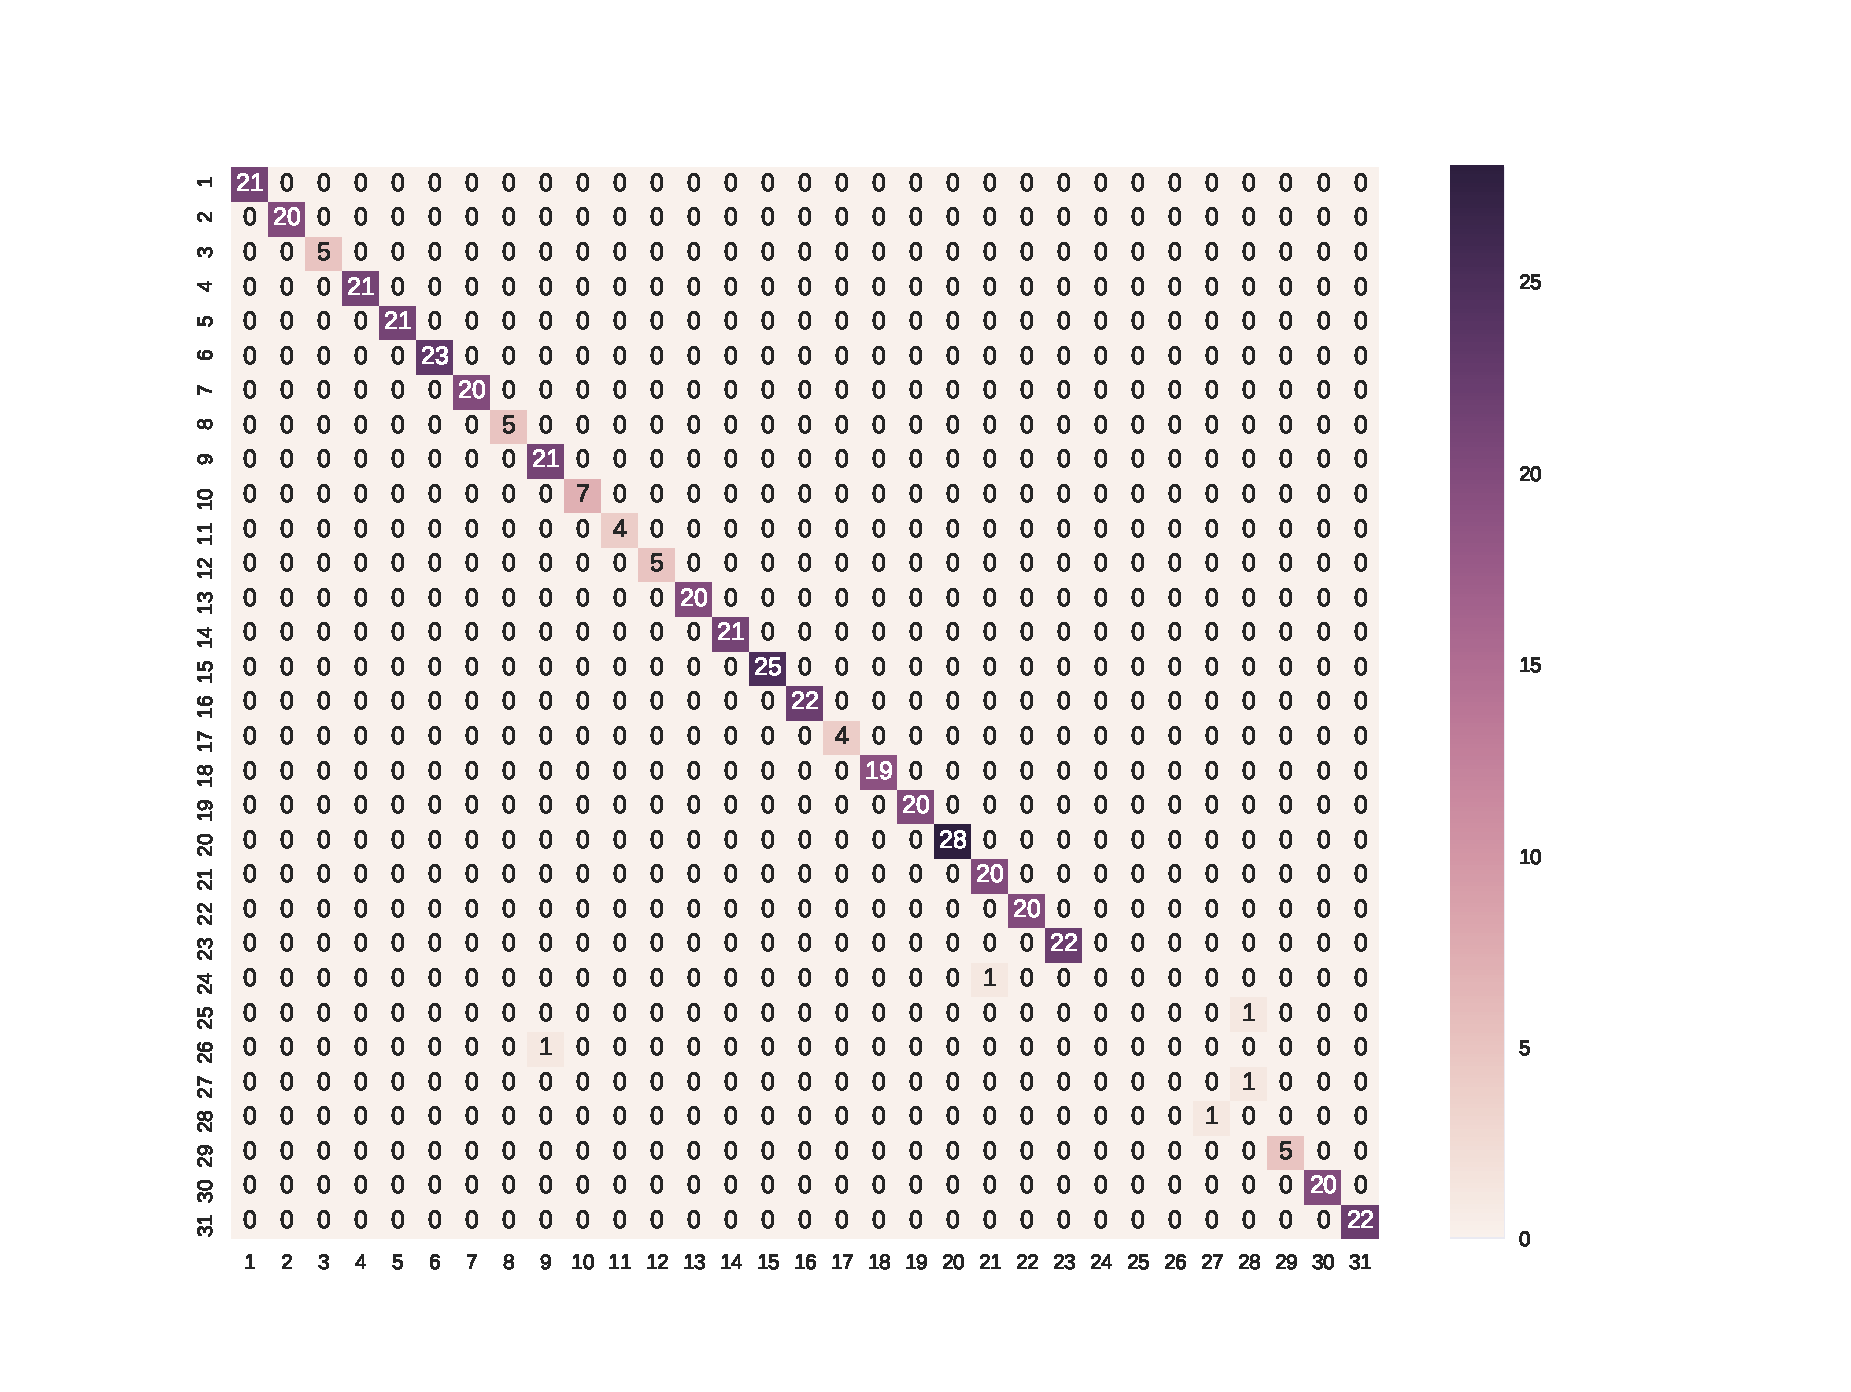
\includegraphics[width=0.8\textwidth]{res/img/resnet_confusion_matrix.pdf}
        \label{subfig:resnet-distance-matrix}
        \caption{Macierz dla~klasyfikatora ResNet.}
    \end{subfigure}
    \caption{Macierze pomyłek dla~obu podejść.
    Wiersze odpowiadają etykietom (identyfikatorom osób) oryginalnych zdjęć,
    kolumny odpowiadają etykietym przypisanym zdjęciom przez klasyfikator.}
\end{figure}

\subsection{Podejście normalizacyjne}

\subsection{Klasyfikator ResNet}

\section{Podsumowanie}

\begin{thebibliography}{9}

    \bibitem{dacosta2016}
        da~Costa-Luis, C. i~inni,
        ,,tqdm''.
        [Online]
        \\
        Dostępne: \url{https://tqdm.github.io/}.
        [Dostęp 11~maja~2019]

    \bibitem{he2015}
        He, K.,
        Zhang, X.,
        Ren, S.,
        Sun, J.,
        ,,Deep Residual Learning for Image Recognition'',
        {\tt arXiv:1512.03385},
        2015.
        [Online]
        \\
        Dostępne: \url{https://arxiv.org/abs/1512.03385}.
        [Dostęp 11~maja~2019]

    \bibitem{hunter2007}
        ,,Matplotlib: A~2D~graphics environment'',
        \emph{Computing In~Science \& Engineering},
        tom~9,
        nr~3,
        s.~90--95,
        2007.

    \bibitem{king2003}
        King, D. i~inni,
        ,,dlib C++ Library''.
        [Online]
        \\
        Dostępne: \url{http://dlib.net/}.
        [Dostęp 11~maja~2019]

    \bibitem{king2015}
        King, D.,
        ,,dlib-models''.
        [Online]
        \\
        Dostępne: \url{https://github.com/davisking/dlib-models}.
        [Dostęp 11~maja~2019]

    \bibitem{mckinney2010}
        McKinney, W.,
        ,,Data Structures for~Statistical Computing in~Python'',
        \emph{Proceedings of~the~9\textsuperscript{th} Python in~Science Conference},
        s.~51--56,
        2010.

    \bibitem{oliphant2006}
        Oliphant, T.E.,
        \emph{A Guide to NumPy},
        Trelgol~Publishing,
        Stany Zjednoczone,
        2006.

    \bibitem{sagonas2013}
        Sagonas, C.,
        Zafeiriou, S.,
        ,,Facial point annotations''.
        [Online]
        \\
        Dostępne: \url{https://ibug.doc.ic.ac.uk/resources/facial-point-annotations/}.
        [Dostęp 11~maja~2019]

    \bibitem{waskom2018}
        Waskom, M. i~inni,
        ,,\texttt{seaborn}: statistical data visualization''.
        [Online]
        \\
        Dostępne: \url{https://seaborn.pydata.org/}.
        [Dostęp 11~maja~2019]

\end{thebibliography}

\end{document}
